	La etapa de salida clase G se caracteriza principalmente por el manejo eficiente de potencia debido a que conmuta la tensión de alimentación entre dos niveles según lo requiera la señal de entrada.

	En la Figura \ref{fig.salida} se muestra un esquema básico de la topología, denominada clase G alternativa.  Los transistores $Q_{63}$ y $Q_{64}$ conforman la etapa interior que opera en clase B, siendo $Q_{14}$ y $Q_{15}$ los \textit{drivers} y sus resistencias de emisor compartidas. 

	%\Juan{Hay que modificar para que coincida con lo de Nico}
	\begin{figure}[H]
		\centering
		\scalebox{0.5}{% XCircuit output "salida.tex" for LaTeX input from salida.eps
\def\putbox#1#2#3#4{\makebox[0in][l]{\makebox[#1][l]{}\raisebox{\baselineskip}[0in][0in]{\raisebox{#2}[0in][0in]{\scalebox{#3}{#4}}}}}
\def\rightbox#1{\makebox[0in][r]{#1}}
\def\centbox#1{\makebox[0in]{#1}}
\def\topbox#1{\raisebox{-0.60\baselineskip}[0in][0in]{#1}}
\def\midbox#1{\raisebox{-0.20\baselineskip}[0in][0in]{#1}}
   \scalebox{1}{
   \normalsize
   \parbox{6.61458in}{
   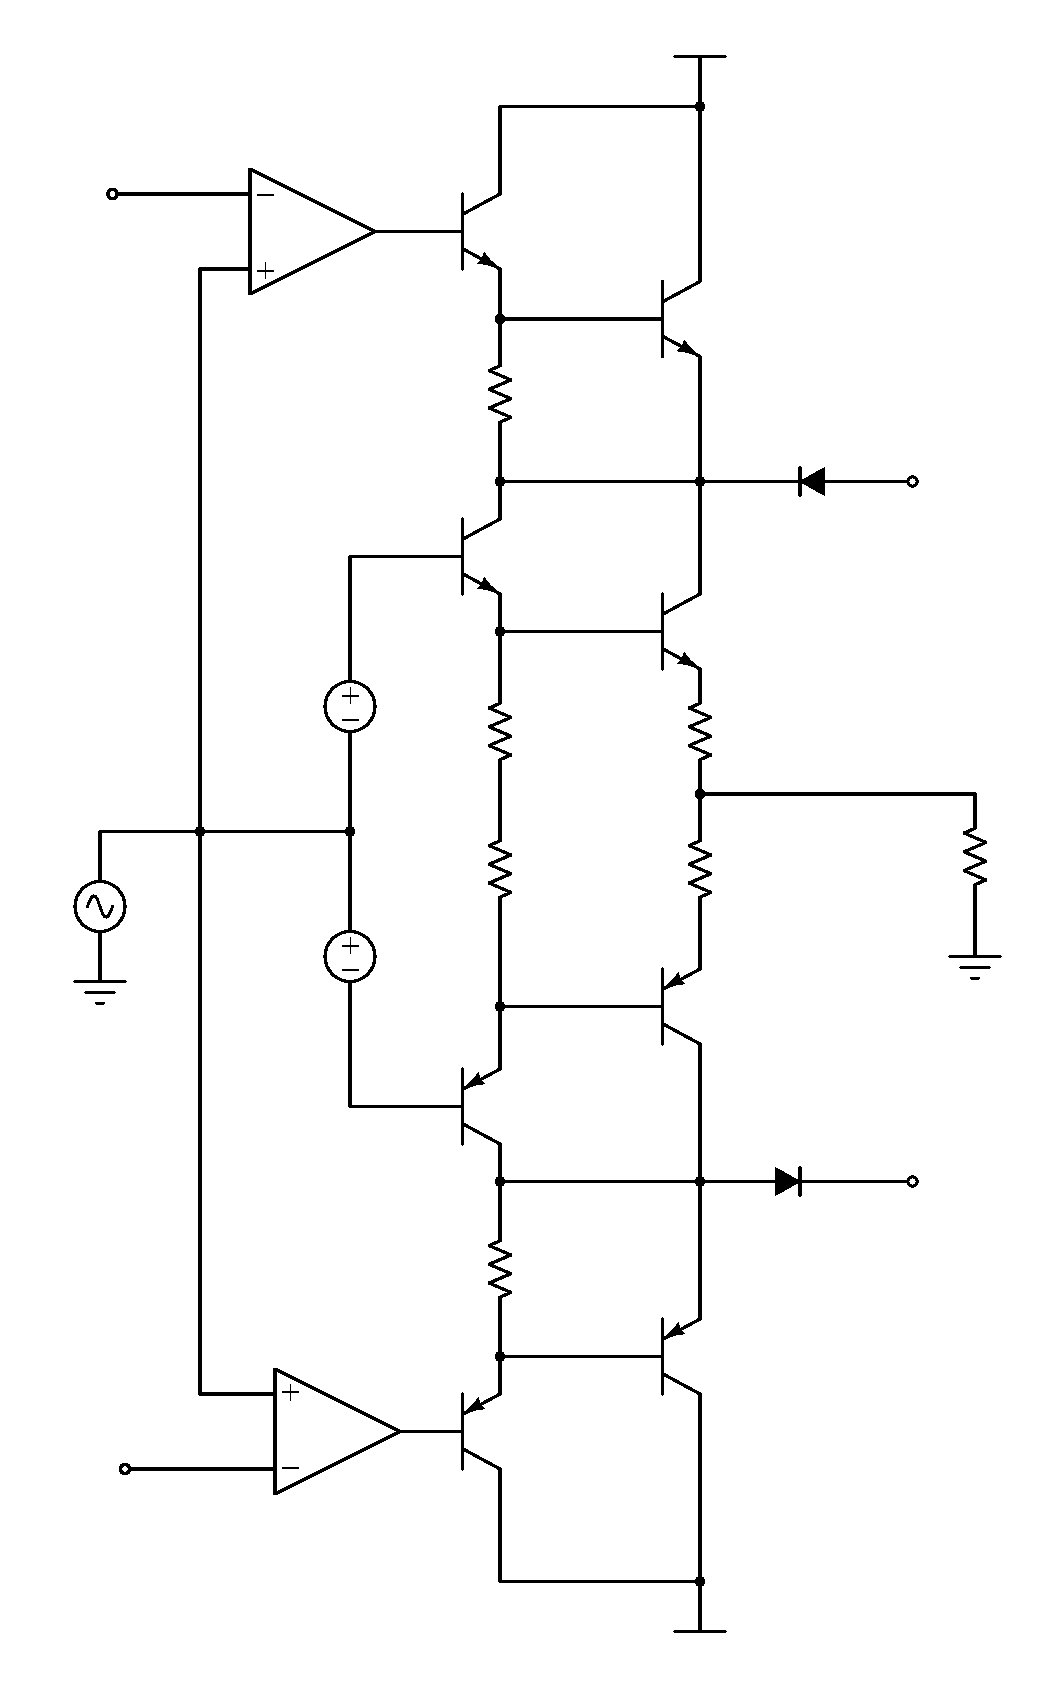
\includegraphics[scale=1]{salida}\\
   % translate x=800 y=1584 scale 0.38
   \putbox{1.39in}{6.39in}{1.20}{Vbias1}%
   \putbox{1.39in}{4.81in}{1.20}{Vbias2}%
   \putbox{5.89in}{5.39in}{1.20}{RL}%
   \putbox{4.72in}{6.22in}{1.20}{Re}%
   \putbox{4.72in}{5.31in}{1.20}{Re}%
   \putbox{4.47in}{6.89in}{1.20}{Q63}%
   \putbox{4.47in}{4.39in}{1.20}{Q64}%
   \putbox{3.14in}{7.47in}{1.20}{Q14}%
   \putbox{3.14in}{3.72in}{1.20}{Q15}%
   \putbox{3.14in}{9.56in}{1.20}{Q16}%
   \putbox{4.47in}{9.06in}{1.20}{Q62}%
   \putbox{3.14in}{1.56in}{1.20}{Q17}%
   \putbox{4.47in}{2.06in}{1.20}{Q65}%
   \putbox{0.14in}{1.31in}{1.20}{Vth-}%
   \putbox{0.06in}{9.81in}{1.20}{Vth+}%
   \putbox{4.22in}{0.06in}{1.20}{-VccH}%
   \putbox{4.22in}{10.89in}{1.20}{+VccH}%
   \putbox{6.06in}{7.89in}{1.20}{VccL+}%
   \putbox{6.06in}{3.22in}{1.20}{-VccL}%
   } % close 'parbox'
   } % close 'scalebox'
   \vspace{-\baselineskip} % this is not necessary, but looks better
}
		\caption{Etapa de salida.}
		\label{fig.salida}
	\end{figure}

	Los comparadores se encuentran conectados a la señal de entrada y a una tensión umbral $V_{th}$ de referencia. Cuando la señal de entrada excede la tensión $+V_{th}$, el comparador (superior) hace que los transistores $Q_{16}$ y $Q_{62}$ se polaricen en saturación. Es decir que actúan como una llave que activa la alimentación $V_{cc_H}$. A su vez el diodo $D_1$ quedará polarizado en inversa ya que la tensión en el cátodo es $+V_{cc_H}$, mayor que la tensión de ánodo $V_{cc_L}$. Por lo tanto, el circuito queda alimentado solo mediante $+V_{cc_H}$ y la potencia es manejada por dos transistores $Q_{62}$ y $Q_{63}$.

	De forma análoga funcionan el comparador inferior, $Q_{17}$, $Q_{65}$ y $D_2$ para el semiciclo negativo de la señal de entrada. La salida se ilustra en la Figura \ref{fig.teo_salida}.


	\HgraficarEPS{0.5}{salidaB}{Forma de la señal de salida, y tensiones umbrales}{fig.teo_salida}
	%\Juan{Hay que modificar para que coincida con lo de Nico}
	\begin{figure}[H]
		\centering
		\scalebox{0.5}{% XCircuit output "salida_2.tex" for LaTeX input from salida_2.eps
\def\putbox#1#2#3#4{\makebox[0in][l]{\makebox[#1][l]{}\raisebox{\baselineskip}[0in][0in]{\raisebox{#2}[0in][0in]{\scalebox{#3}{#4}}}}}
\def\rightbox#1{\makebox[0in][r]{#1}}
\def\centbox#1{\makebox[0in]{#1}}
\def\topbox#1{\raisebox{-0.60\baselineskip}[0in][0in]{#1}}
\def\midbox#1{\raisebox{-0.20\baselineskip}[0in][0in]{#1}}
   \scalebox{1}{
   \normalsize
   \parbox{6.61458in}{
   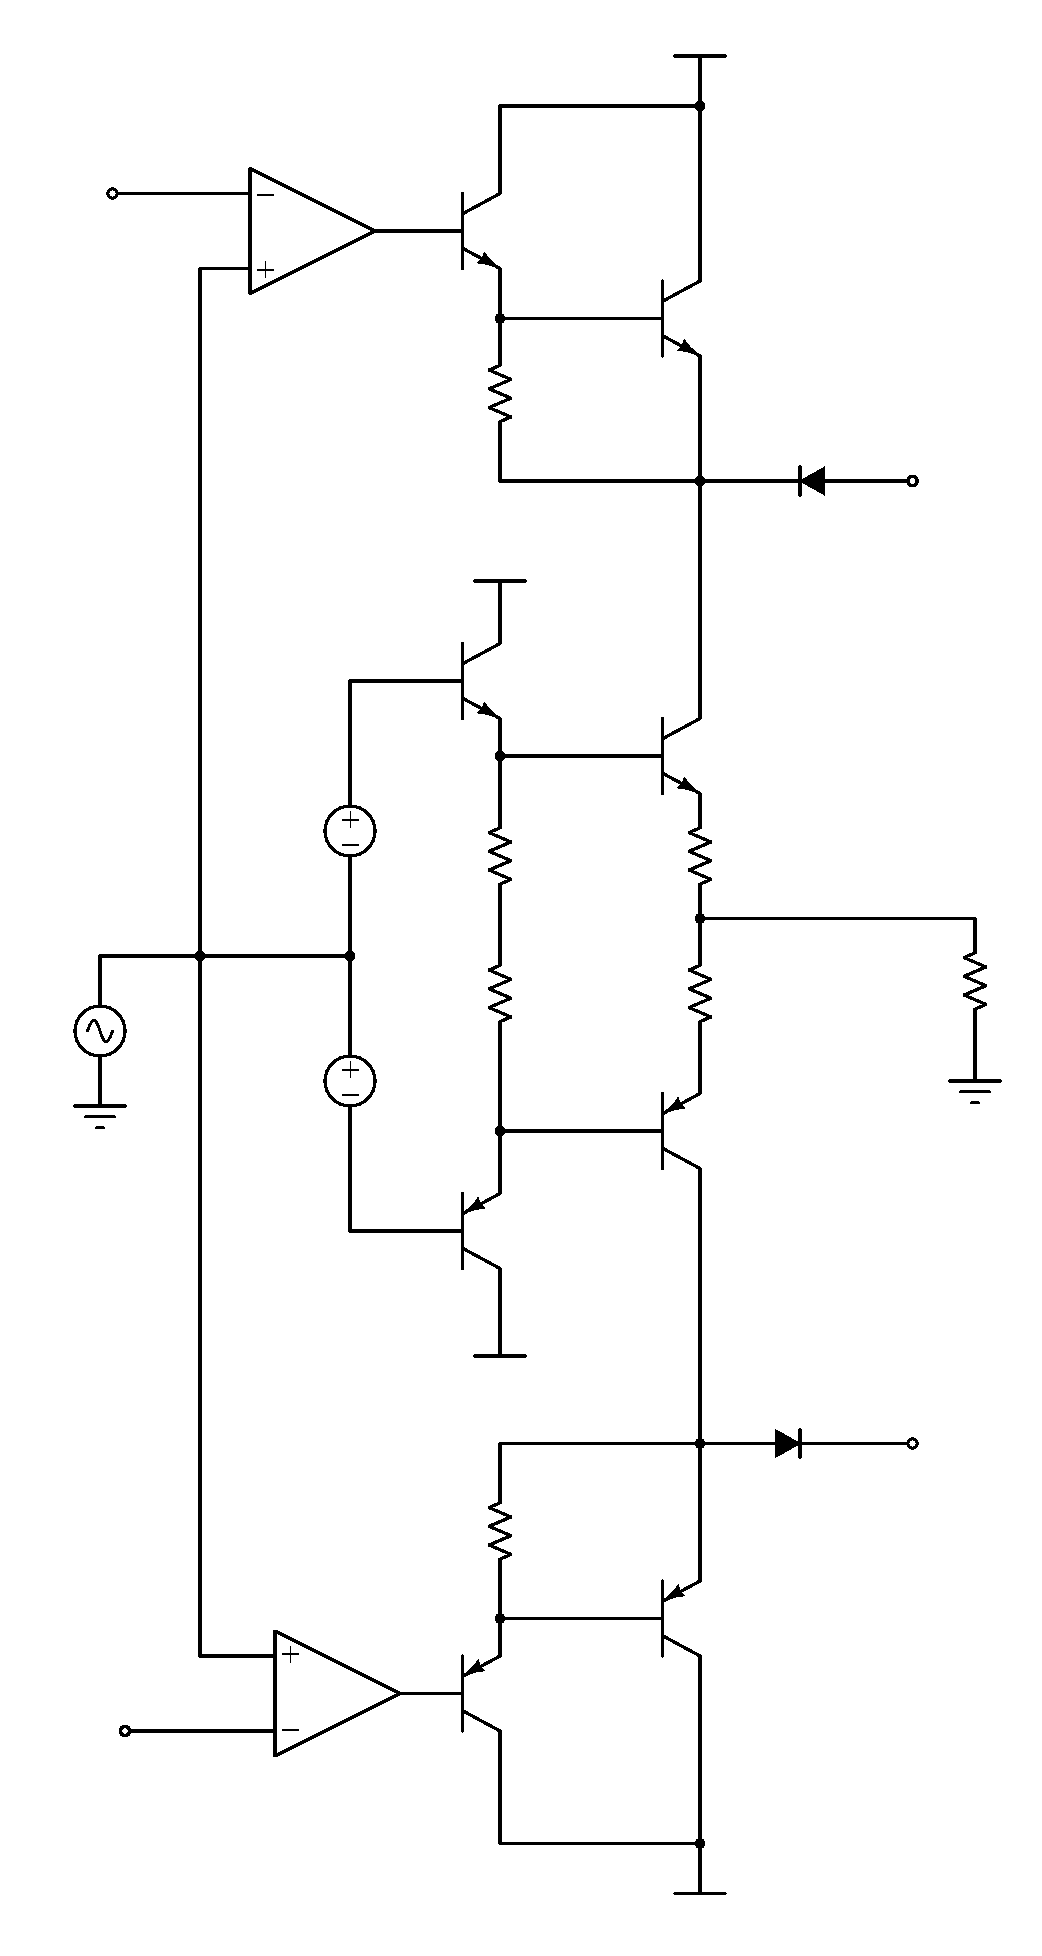
\includegraphics[scale=1]{salida_2}\\
   % translate x=800 y=1760 scale 0.38
   \putbox{1.39in}{7.31in}{1.20}{Vbias1}%
   \putbox{1.39in}{5.72in}{1.20}{Vbias2}%
   \putbox{5.89in}{6.31in}{1.20}{RL}%
   \putbox{4.72in}{7.14in}{1.20}{Re}%
   \putbox{4.72in}{6.22in}{1.20}{Re}%
   \putbox{4.47in}{7.81in}{1.20}{Q63}%
   \putbox{4.47in}{5.31in}{1.20}{Q64}%
   \putbox{3.14in}{8.39in}{1.20}{Q14}%
   \putbox{3.14in}{4.64in}{1.20}{Q15}%
   \putbox{3.14in}{11.31in}{1.20}{Q16}%
   \putbox{4.47in}{10.81in}{1.20}{Q62}%
   \putbox{3.14in}{1.56in}{1.20}{Q17}%
   \putbox{4.47in}{2.06in}{1.20}{Q65}%
   \putbox{0.14in}{1.31in}{1.20}{Vth-}%
   \putbox{0.06in}{11.56in}{1.20}{Vth+}%
   \putbox{4.22in}{0.06in}{1.20}{-VccH}%
   \putbox{4.22in}{12.64in}{1.20}{+VccH}%
   \putbox{6.06in}{9.64in}{1.20}{VccL+}%
   \putbox{6.06in}{3.22in}{1.20}{-VccL}%
   \putbox{2.89in}{9.14in}{1.20}{+VccH}%
   \putbox{2.89in}{3.64in}{1.20}{-VccH}%
   } % close 'parbox'
   } % close 'scalebox'
   \vspace{-\baselineskip} % this is not necessary, but looks better
}
		\caption{Topología final de la etapa de salida.}
		\label{fig.salida_2}
	\end{figure}
	Sin embargo, la topología propuesta en la Figura \ref{fig.salida} presenta un inconveniente. Cuando $Q_{62}$ entra en conducción, se produce una alteración repentina en la tensión $V_{CE}$ del transistor de potencia de salida $Q_1$, que por efecto Early también modifica la corriente de colector. Esta alteración afecta la ganancia, produciendo picos de tensión en la señal de salida. Esta alinealidad se elimina al conectar los transistores internos $Q_{14}$ y $Q_{15}$ a la tensión $+V_{cc_H}$ y $-V_{cc_H}$ respectivamente, según indica la Figura \ref{fig.salida_2}.

\subsection{Multiplicador de $V_{BE}$}

Las tensiones $V_{bias1}$ y $V_{bias2}$ permiten \textit{prepolarizar} a los transistores $Q_{63}$ y $Q_{64}$ con el fin de atenuar la distorsión de cruce por cero característica del clase B. Se deben ajustar de forma tal que la corriente de la malla de salida sea aproximadamente igual en el colector de ambos transistores ($Q_{63}$ y $Q_{64}$). Asimismo se debe considerar que si $I_{CQ}$ es muy elevada se desperdicia potencia, y si es muy pequeña se obtendrá una distorsión de cruce por cero apreciable. Ambas tensiones se implementaron con un multiplicador de $V_{BE}$ cuyo circuito se presenta en la Figura \ref{fig.multiplicador}.

	%\Juan{Idem}
	\begin{figure}[H]
		\centering
		\scalebox{0.5}{% XCircuit output "multiplicador.tex" for LaTeX input from multiplicador.eps
\def\putbox#1#2#3#4{\makebox[0in][l]{\makebox[#1][l]{}\raisebox{\baselineskip}[0in][0in]{\raisebox{#2}[0in][0in]{\scalebox{#3}{#4}}}}}
\def\rightbox#1{\makebox[0in][r]{#1}}
\def\centbox#1{\makebox[0in]{#1}}
\def\topbox#1{\raisebox{-0.60\baselineskip}[0in][0in]{#1}}
\def\midbox#1{\raisebox{-0.20\baselineskip}[0in][0in]{#1}}
   \scalebox{1}{
   \normalsize
   \parbox{4.18229in}{
   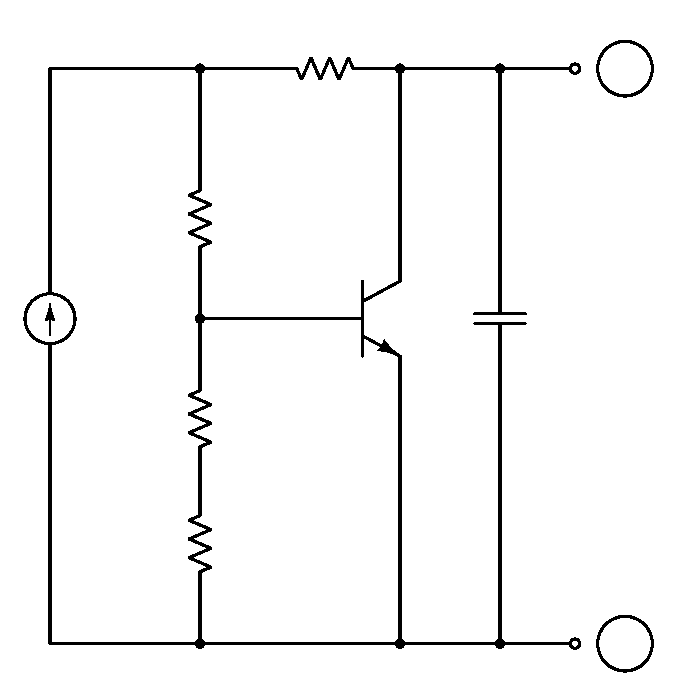
\includegraphics[scale=1]{multiplicador}\\
   % translate x=672 y=611 scale 0.38
   \putbox{3.56in}{2.32in}{1.20}{C20}%
   \putbox{2.47in}{2.32in}{1.20}{Q26}%
   \putbox{0.56in}{3.07in}{1.20}{R43}%
   \putbox{0.72in}{1.74in}{1.20}{Rp}%
   \putbox{0.64in}{0.82in}{1.20}{R44}%
   \putbox{1.89in}{4.24in}{1.20}{R42}%
   \putbox{4.06in}{4.07in}{1.20}{\centbox{\midbox{1,1}}}%
   \putbox{4.06in}{0.24in}{1.20}{\centbox{\midbox{-1,1}}}%
   \putbox{0.47in}{2.32in}{1.20}{Ipol}%
   \putbox{1.97in}{3.74in}{1.20}{$10 \Omega$}%
   \putbox{1.47in}{3.07in}{1.20}{$3,3 k\Omega$}%
   \putbox{1.39in}{0.82in}{1.20}{$680 \Omega$}%
   \putbox{1.39in}{1.65in}{1.20}{$1 k\Omega$}%
   } % close 'parbox'
   } % close 'scalebox'
   \vspace{-\baselineskip} % this is not necessary, but looks better
}
		\caption{Multiplicador de $V_{BE}$.}
		\label{fig.multiplicador}
	\end{figure}


	\begin{equation}
		\centering
		V_M = \left( \frac{R_{43}}{R_{43} + R_{44}} +1 \right) \cdot V_{BE} - I_C \cdot R_{42} \approx  \left( \frac{R_{43}}{R_{43} + R_{44}} +1 \right) \cdot V_{BE}
	\end{equation}

	 Considerando un valor de $V_{BE} \approx \SI{0.5}{\volt}$

	 \begin{equation}
	 	\centering
		\frac{\SI{2.2}{\volt}}{\SI{0.5}{\volt}} -1 = \frac{R_{43}}{R_{44}} \implies \boxed{R_{43} = \num{3,4} \cdot R_{44}}
	\end{equation}

	Se eligen los resistores comerciales $R_{43} = \SI{3.3}{\kilo\ohm}$, $R_{44} = \SI{680}{\ohm}$ y un potenciómetro de $\SI{1}{\kilo\ohm}$. 

	La resistencia $R_{42}$ se anexa para mejorar la independencia de la tensión $V_{CE}$ con la corriente de polarización. Asimismo se agrega un capacitor $C_M$ para no alterar el comportamiento del resto circuito en señal, es decir que se obtiene una impedancia pequeña para un amplio rango de frecuencias. 
	
\subsection{Compensación del embalamiento térmico}

	Se logra al agregar una resistencia al emisor de cada transistor equivalente de la etapa de salida. Si la señal de entrada se encuentra en su semiciclo positivo, sólo el transistor equivalente formado por $Q_{63}$ y $Q_{14}$ conduce. Ante un aumento de la temperatura, se produce un incremento de la corriente de colector, por ende aumenta la caída de tensión en $R_{32}$, entonces necesariamente la tensión $V_{BE}$ disminuye, produciendo un decremento en la corriente de colector. De esta manera se logra estabilizar la polarización de la etapa de salida mediante realimentación negativa local. El valor de dichas resistencias ($R_{32}$ y $R_{33}$) debe ser pequeño en comparación al valor de la carga con el fin de no alterar la tensión útil de salida. Asimismo para que la realimentación sea suficiente se debe cumplir la expresión \eqref{ec.re1}:

\begin{equation}
	\centering
	R_E \geq \frac{\Theta_{ja,Q_{63}} V_{CC} \cdot \SI{2}{\milli\volt\per\celsius}}{\beta_{min} + 1}
	\label{ec.re1}
\end{equation}
	
	Se utilizarán como transistores de salida los \texttt{2SC5198} y \texttt{2SA1941}. A partir de la hoja de datos, se obtiene $\Theta_{ja,Q_{63}} = \SI{150}{\celsius\per\watt}$ y $\beta_{min} = 35$, por lo que se obtiene el valor mínimo para $R_E$ es \eqref{ec.re}.

	\begin{equation}
		\centering
		R_E \geq \frac{ \SI{150}{\celsius\per\watt} \cdot \SI{40}{\volt} \cdot \SI{2}{\milli\volt\per\celsius} }{ 35 + 1 } = \SI{0.33}{\ohm}
		\label{ec.re}
	\end{equation}



	\subsection{Protección}
	Se implementó una protección contra cortocircuito de la carga de salida, conformado por los transistores $Q_{52}$ y $Q_{53}$. Dicho circuito sensa la corriente de salida y si supera cierto umbral, la tensión de $V_{BE}$ resulta lo suficientemente elevada como para que el transistor $Q_{53}$ entre en conducción. De esta manera la corriente que circularía por los transistores de salida se desvía hacia los transistores de protección.
	Dicho circuito se expone en la Figura \ref{fig.proteccion}.
%
%	\begin{figure}[H]
%		\centering
%		\scalebox{0.5}{% XCircuit output "proteccion.tex" for LaTeX input from proteccion.eps
\def\putbox#1#2#3#4{\makebox[0in][l]{\makebox[#1][l]{}\raisebox{\baselineskip}[0in][0in]{\raisebox{#2}[0in][0in]{\scalebox{#3}{#4}}}}}
\def\rightbox#1{\makebox[0in][r]{#1}}
\def\centbox#1{\makebox[0in]{#1}}
\def\topbox#1{\raisebox{-0.60\baselineskip}[0in][0in]{#1}}
\def\midbox#1{\raisebox{-0.20\baselineskip}[0in][0in]{#1}}
   \scalebox{1}{
   \normalsize
   \parbox{4.66667in}{
   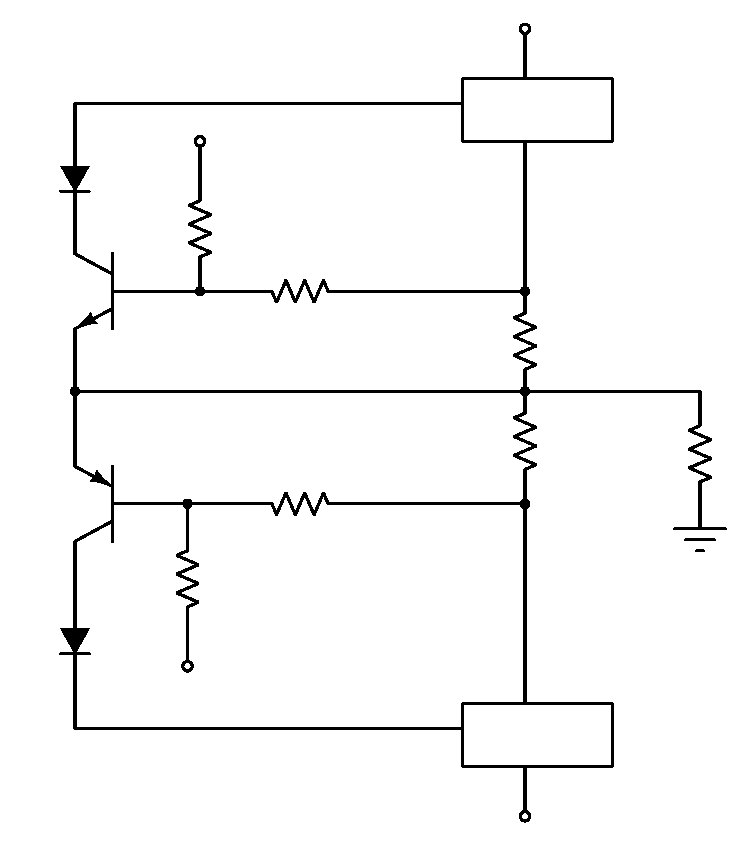
\includegraphics[scale=1]{proteccion}\\
   % translate x=3040 y=-1322 scale 0.38
   \putbox{3.14in}{4.84in}{1.20}{Etapa}%
   \putbox{3.06in}{4.67in}{1.20}{de salida}%
   \putbox{3.14in}{0.67in}{1.20}{Etapa}%
   \putbox{3.06in}{0.50in}{1.20}{de salida}%
   \putbox{4.14in}{2.42in}{1.20}{RL}%
   \putbox{3.64in}{3.50in}{1.20}{Re}%
   \putbox{3.56in}{2.50in}{1.20}{Re}%
   \putbox{0.72in}{4.00in}{1.20}{R60}%
   \putbox{1.72in}{3.75in}{1.20}{R59}%
   \putbox{1.72in}{2.34in}{1.20}{R57}%
   \putbox{1.31in}{1.67in}{1.20}{R58}%
   \putbox{0.06in}{3.50in}{1.20}{Q52}%
   \putbox{0.06in}{2.09in}{1.20}{Q53}%
   \putbox{1.39in}{4.00in}{1.20}{22k}%
   \putbox{1.72in}{3.34in}{1.20}{270}%
   \putbox{1.72in}{1.92in}{1.20}{270}%
   \putbox{0.72in}{1.59in}{1.20}{22k}%
   } % close 'parbox'
   } % close 'scalebox'
   \vspace{-\baselineskip} % this is not necessary, but looks better
}
%		\caption{Protección contra cortocircuito en la salida.}
%		\label{fig.proteccion}
%	\end{figure}
%	\Flor{Este anda bien en simulación, con 2k2 en vez de 1k8.}
	\begin{figure}[H]
		\centering
		\scalebox{0.5}{% XCircuit output "proteccion2.tex" for LaTeX input from proteccion2.eps
\def\putbox#1#2#3#4{\makebox[0in][l]{\makebox[#1][l]{}\raisebox{\baselineskip}[0in][0in]{\raisebox{#2}[0in][0in]{\scalebox{#3}{#4}}}}}
\def\rightbox#1{\makebox[0in][r]{#1}}
\def\centbox#1{\makebox[0in]{#1}}
\def\topbox#1{\raisebox{-0.60\baselineskip}[0in][0in]{#1}}
\def\midbox#1{\raisebox{-0.20\baselineskip}[0in][0in]{#1}}
   \scalebox{1}{
   \normalsize
   \parbox{4.66667in}{
   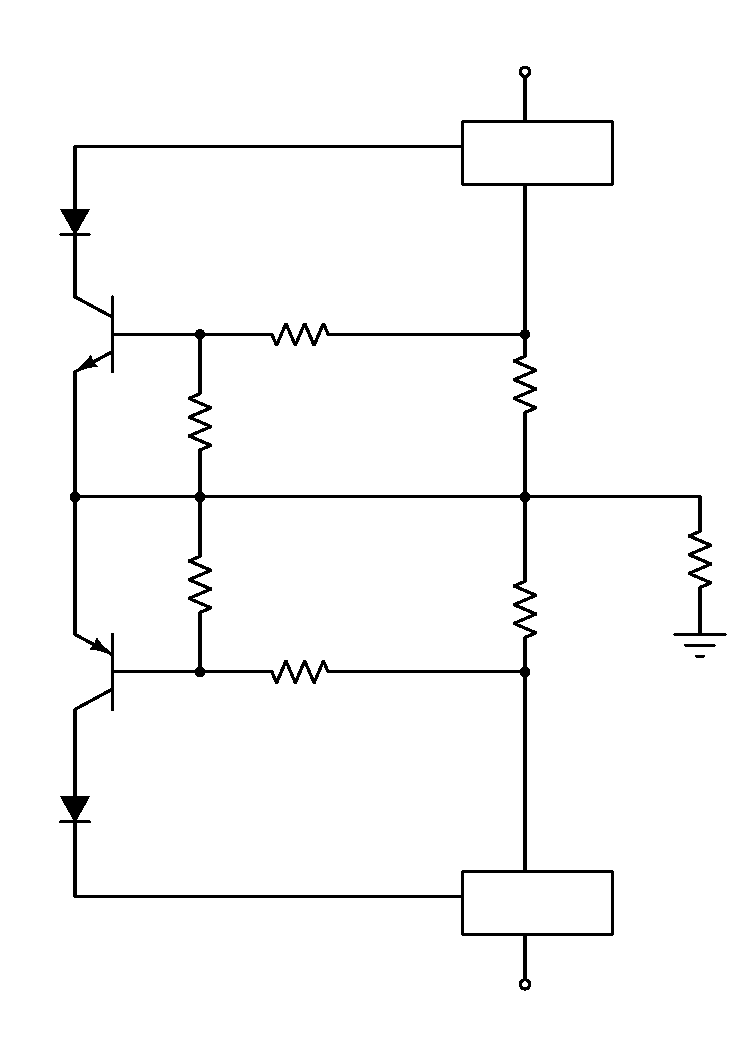
\includegraphics[scale=1]{proteccion2}\\
   % translate x=3040 y=-1116 scale 0.38
   \putbox{3.14in}{5.91in}{1.20}{Etapa}%
   \putbox{3.06in}{5.74in}{1.20}{de salida}%
   \putbox{3.14in}{0.91in}{1.20}{Etapa}%
   \putbox{3.06in}{0.74in}{1.20}{de salida}%
   \putbox{4.14in}{3.08in}{1.20}{RL}%
   \putbox{3.64in}{4.24in}{1.20}{Re}%
   \putbox{3.56in}{2.74in}{1.20}{Re}%
   \putbox{0.72in}{4.08in}{1.20}{R60}%
   \putbox{1.72in}{4.83in}{1.20}{R59}%
   \putbox{1.72in}{2.58in}{1.20}{R57}%
   \putbox{0.72in}{2.91in}{1.20}{R58}%
   \putbox{0.06in}{4.58in}{1.20}{Q52}%
   \putbox{0.06in}{2.33in}{1.20}{Q53}%
   \putbox{1.39in}{4.08in}{1.20}{1k}%
   \putbox{1.72in}{4.41in}{1.20}{1k8}%
   \putbox{1.72in}{2.16in}{1.20}{1k8}%
   \putbox{1.39in}{2.91in}{1.20}{1k}%
   \putbox{3.39in}{6.58in}{1.20}{\centbox{$V_{CC+}$}}%
   \putbox{3.39in}{0.08in}{1.20}{\centbox{$V_{CC-}$}}%
   } % close 'parbox'
   } % close 'scalebox'
   \vspace{-\baselineskip} % this is not necessary, but looks better
}
		\caption{Protección contra cortocircuito en la salida.}
		\label{fig.proteccion}
	\end{figure}


	La máxima diferencia de potencial que habrá sobre $R_L$ es $V_{CCL+} - V^{Q_{63}}_{CE_{sat}}$ cuando se opera con $V_{CCL+}$ y $V_{CCH+} - V^{Q_{62}}_{CE_{sat}} - V^{Q_{63}}_{CE_{sat}}$ para tensiones mayores a $V_{CCL+}$. Se puede ver que el peor caso es cuando las tensiones son mayores a $V_{CCL+}$ y por lo tanto (suponiendo $V_{CE_{sat}} \approx V_{BE_{ON}} \approx \SI{0.6}{\V}$) la potencia máxima que disipará la carga es:
		\begin{equation*}
			P_{RL_{\max}} = \frac{\left(V_{CCH+} - V^{Q_{62}}_{CE_{sat}} - V^{Q_{63}}_{CE_{sat}}\right)^2}{R_L} = \frac{\left(\SI{30}{\V} - \SI{1.2}{\V}\right)^2}{\SI{8}{\ohm}} = \SI{104}{\W}
		\end{equation*}

	De este modo la máxima corriente que circula sobre los transistores de salida es
		\begin{equation*}
			\boxed{I_{O_{\max}} = \frac{P_{RL_{\max}}}{V_{CCH+}} = \SI{3.5}{\A}}
		\end{equation*}

%	Si se configurase al circuito protector de tal forma que al alcanzar dicho valor corte el circuito, no se podrá obtener la máxima potencia con baja distorsión dado que la característica de los transistores es exponencial y por tanto al acercarse al valor de corte comenzará a extraer corriente del multiplicador de $V_{BE}$. Es por tanto que se propone como peor caso que la fuente varíe positivamente un 20\%, es decir $V_{CCH+}=\SI{40}{\V}$. Realizando los mismos cálculos se optiene $I_{O_{\max}} = \SI{4.65}{\A}$. \\
%	Para dicha corriente y $R_{E} = \SI{.33}{\ohm}$ se obtiene $V_{E} = \SI{1.535}{\V}$. Así se halla que la relación entre las resistencias del divisor resistivo es de 433. Se propone entonces los valores de componentes de la Figura \ref{fig.proteccion} que se consiguen comercialmente obteninedose efectivamente $I_{O_{\max}}=\SI{4.63}{\A}$.


	Si se configurase al circuito protector de tal forma que al alcanzar dicho valor corte el circuito, no se podrá obtener la máxima potencia con baja distorsión dado que la característica de los transistores es exponencial y por tanto al acercarse al valor de corte comenzará a extraer corriente del multiplicador de $V_{BE}$. Por otra parte, debido a que la fuente de alimetnación puede variar positivamente en un 20\%, es decir $V_{CCH+}=\SI{40}{\V}$, y que la resistencia equivalente de la carga puede ser menor que \SI{8}{\ohm}, se propone que el circuito de protección se active cuando en la salida circulen $\SI{5}{\ampere}$.

	Para dicha corriente y $R_{E} = \SI{.33}{\ohm}$ se obtiene $V_{E} = \SI{1.65}{\V}$. Así se halla que la relación entre las resistencias del divisor resistivo es de \num{1,8}. Se propone entonces los valores de componentes de la Figura \ref{fig.proteccion} que se consiguen comercialmente.

	\begin{align}
		\centering
		\Delta V_{Re} &= \SI{0.33}{\ohm} \cdot \SI{5}{\ampere} = \SI{1.65}{\volt} \\
		\SI{0.6}{\volt} &= \frac{R_{60}}{ R_{60} + R_{59} } \cdot \SI{1.65}{\volt} \implies \boxed{R_{59} = \num{1,8} \: R_{60}}
	\end{align}

		

\subsection{Fuente de corriente}
	De la sección anterior se sabe que $I_{O_{\max}}=\SI{3.5}{\A}$. Al tratarse de transistores de potencia, el factor $\beta$ se encuentra entre 30 y 50, por lo que la corriente de base en $Q_{63}$ sería $I_{B,Q63} \approx \SI{100}{\milli\ampere}$. Dicha corriente es entregada por $Q_{14}$, siendo la corriente de base $I_{B,Q14} \approx \SI{2}{\milli\ampere}$. A su vez la fuente polariza la etapa amplificadora de tensión (VAS), por lo que se considerará al menos un cuarto más de dicha corriente. Se propone $I_{pol} = \SI{5}{\milli\ampere}$.

	\begin{figure}[H]
		\centering
		\scalebox{0.5}{% XCircuit output "fte.tex" for LaTeX input from fte.eps
\def\putbox#1#2#3#4{\makebox[0in][l]{\makebox[#1][l]{}\raisebox{\baselineskip}[0in][0in]{\raisebox{#2}[0in][0in]{\scalebox{#3}{#4}}}}}
\def\rightbox#1{\makebox[0in][r]{#1}}
\def\centbox#1{\makebox[0in]{#1}}
\def\topbox#1{\raisebox{-0.60\baselineskip}[0in][0in]{#1}}
\def\midbox#1{\raisebox{-0.20\baselineskip}[0in][0in]{#1}}
   \scalebox{1}{
   \normalsize
   \parbox{3.85938in}{
   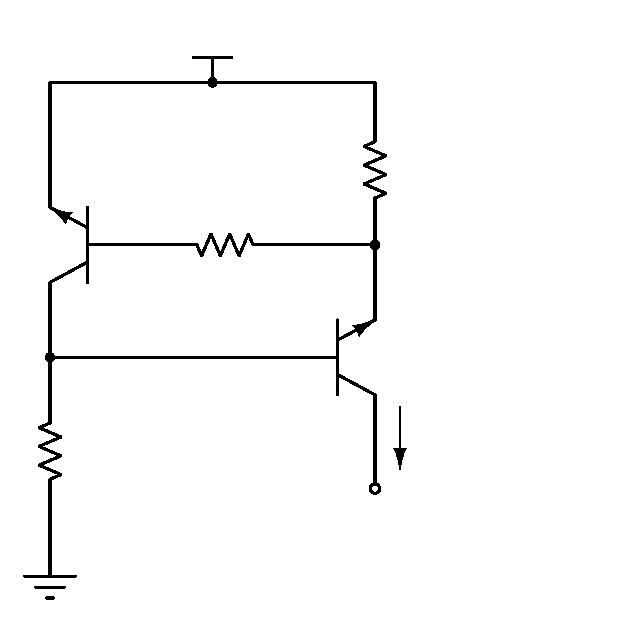
\includegraphics[scale=1]{fte}\\
   % translate x=384 y=372 scale 0.38
   \putbox{0.43in}{0.91in}{1.20}{$20 k\Omega$}%
   \putbox{2.56in}{2.83in}{1.20}{$100 \Omega$}%
   \putbox{1.47in}{2.54in}{1.20}{$2,2 k\Omega$}%
   \putbox{2.76in}{1.16in}{1.20}{$5 mA$}%
   \putbox{0.97in}{3.74in}{1.20}{VccH+}%
   \putbox{1.97in}{2.87in}{1.20}{R1}%
   \putbox{1.01in}{2.54in}{1.20}{R2}%
   \putbox{2.81in}{0.83in}{1.20}{$I_{pol}$}%
   \putbox{0.51in}{2.87in}{1.20}{$V_{BE}$}%
   \putbox{1.18in}{1.83in}{1.20}{$V_{BE}$}%
   \putbox{0.72in}{2.16in}{1.20}{\textcolor{blue}{$30V-V_{BE}$}}%
   } % close 'parbox'
   } % close 'scalebox'
   \vspace{-\baselineskip} % this is not necessary, but looks better
}
		\caption{Fuente de corriente.}
		\label{fig.fte}
	\end{figure}

\begin{equation}
	\centering
	R_6 = \frac{\SI{30}{\volt} - V_{BE, <on>} }{ I_{pol} }
	\label{ec.ipol}
\end{equation}

La corriente de polarización queda determinada por la resistencia $R_6$ de la Ecuación \ref{ec.ipol}. Considerando un $V_{BE,on} = \SI{0.5}{\volt}$ se obtiene $R_6 = \SI{100}{\ohm}$. Por otra parte se despreció la caída de tensión por $R_5$. Dicha resistencia se anexa con el fin de limitar la corriente de base que pasa de un transistor a otro.


\subsection{Comparadores}

	Las señales de música poseen picos de tensión cuya magnitud es mucho mayor al valor medio, estando la mayor parte del tiempo en niveles bajos, por lo que se propone un umbral de tensión de 40\% con respecto a la tensión máxima de alimentación, es decir que $V_{cc_L} = \pm \SI{12}{\volt}$, $V_{cc_H} = \pm \SI{30}{\volt}$.

	\begin{figure}[H]
		\centering
		\scalebox{0.5}{% XCircuit output "comparador.tex" for LaTeX input from comparador.eps
\def\putbox#1#2#3#4{\makebox[0in][l]{\makebox[#1][l]{}\raisebox{\baselineskip}[0in][0in]{\raisebox{#2}[0in][0in]{\scalebox{#3}{#4}}}}}
\def\rightbox#1{\makebox[0in][r]{#1}}
\def\centbox#1{\makebox[0in]{#1}}
\def\topbox#1{\raisebox{-0.60\baselineskip}[0in][0in]{#1}}
\def\midbox#1{\raisebox{-0.20\baselineskip}[0in][0in]{#1}}
   \scalebox{1}{
   \normalsize
   \parbox{7.08333in}{
   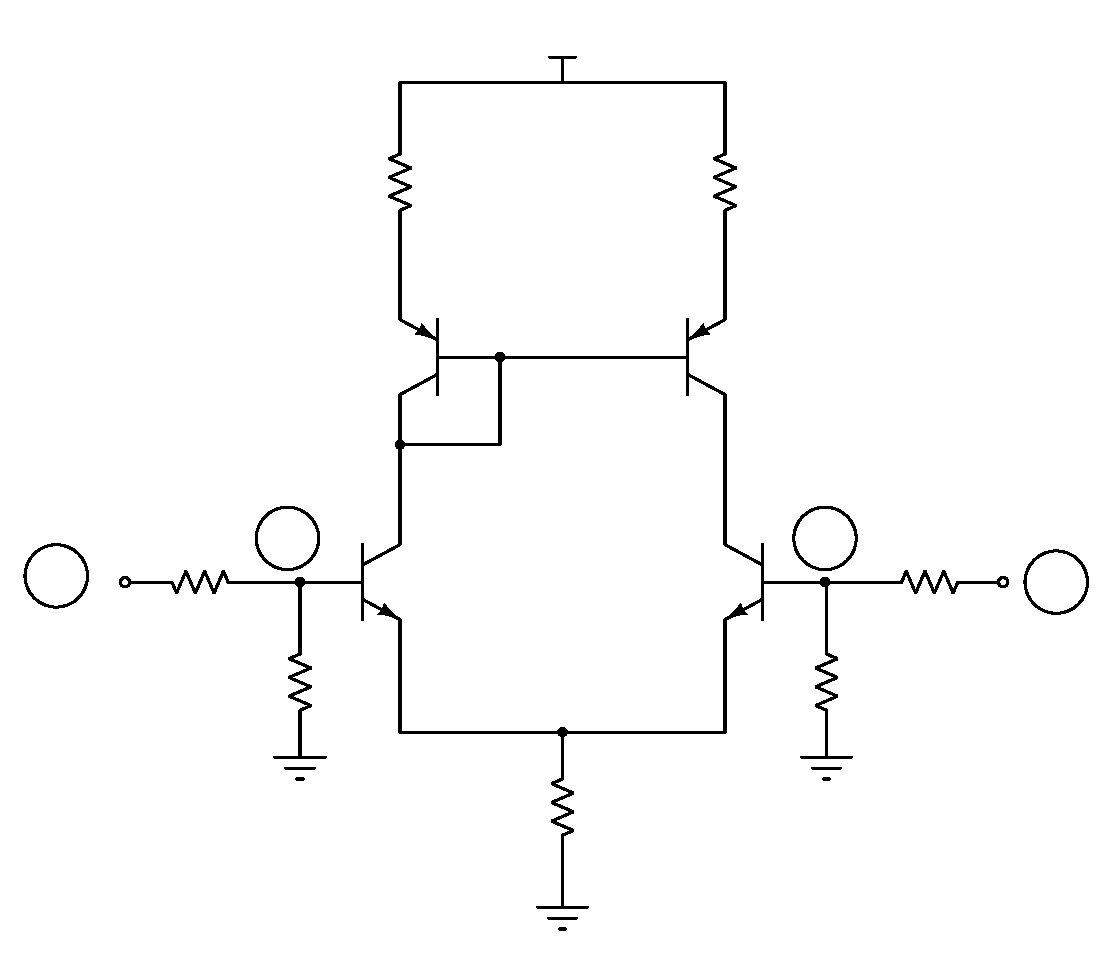
\includegraphics[scale=1]{comparador}\\
   % translate x=928 y=636 scale 0.38
   \putbox{2.58in}{2.33in}{1.20}{Q9}%
   \putbox{4.45in}{2.29in}{1.20}{Q10}%
   \putbox{2.37in}{3.81in}{1.20}{Q11}%
   \putbox{4.66in}{3.81in}{1.20}{Q12}%
   \putbox{3.35in}{5.95in}{1.20}{+VccH}%
   \putbox{0.14in}{2.33in}{1.20}{Vo}%
   \putbox{3.18in}{0.83in}{1.20}{Rec}%
   \putbox{1.10in}{2.54in}{1.20}{R1}%
   \putbox{1.47in}{1.70in}{1.20}{R2}%
   \putbox{5.97in}{2.49in}{1.20}{R3}%
   \putbox{5.01in}{1.66in}{1.20}{R4}%
   \putbox{2.18in}{5.04in}{1.20}{R5}%
   \putbox{4.35in}{4.99in}{1.20}{R6}%
   \putbox{1.64in}{2.58in}{1.20}{Vo'}%
   \putbox{5.18in}{2.58in}{1.20}{Vth'}%
   \putbox{6.76in}{2.33in}{1.20}{Vth}%
   \putbox{2.76in}{5.04in}{1.20}{56}%
   \putbox{4.93in}{5.04in}{1.20}{56}%
   \putbox{1.10in}{2.08in}{1.20}{5,6k}%
   \putbox{2.06in}{1.70in}{1.20}{1k}%
   \putbox{5.51in}{1.70in}{1.20}{1k}%
   \putbox{5.89in}{2.08in}{1.20}{8,2k}%
   \putbox{3.81in}{0.83in}{1.20}{560}%
   } % close 'parbox'
   } % close 'scalebox'
   \vspace{-\baselineskip} % this is not necessary, but looks better
}
		\caption{Comparador.}
		\label{fig.comparador}
	\end{figure}

	Se propone la configuración de par diferencial de la Figura \ref{fig.comparador} para implementar los comparadores. Se utiliza una carga espejo para lograr mayor estabilidad. Además en vez de comparar con la señal proveniente de la etapa VAS, se compara con la señal de salida $V_{o}$ para evitar cargar dicha etapa con la resistencia de entrada que presenta el par diferencial ($2\cdot r_\pi$). La señal de salida no resulta alterada por tratarse de un colector común que es separador de impedancias (nodo de baja impedancia).\\
	\indent Por otra parte, es difícil lograr en la práctica que los transistores que conforman el par diferencial manejen una excursión de tensión de hasta \SI{30}{\volt}, por lo que se utiliza un divisor resistivo en ambas bases de los transistores para atenuar la amplitud de tensión. Es conveniente que la tensión de referencia $V_{th}'$ sea levemente menor que la prevista con el fin de contrarrestar el retardo de tiempo del comparador.

\begin{equation}
	\centering
	V_{th}' = V_{th} \cdot \frac{R_{63}}{R_{63} + R_{64}} \implies \SI{1.5}{\volt} = \SI{12}{\volt} \cdot \frac{R_{63}}{R_{63} + R_{64}} \implies \boxed{R_{64} = 7 \cdot R_{63}}
\end{equation}

\begin{equation}
	\centering
	V_o' = V_o \cdot \frac{R_{62}}{R_{62} + R_{61}} \implies \SI{2}{\volt} = \SI{12}{\volt} \cdot \frac{R_{62}}{R_{62} + R_{61}} \implies \boxed{R_{61} = 5 \cdot R_{62}}
	\end{equation}

	El valor de la resistencia de emisor $R_{51}$ se elige en función de la máxima tensión posible en $V_o$ y la corriente que circularía en reposo. Con $R_{51} = \SI{500}{\ohm}$ se obtiene:

	\begin{equation}
		\centering
		I_{e,\max} = \frac{ \SI{1.3}{\volt} }{ \SI{500}{\ohm} } = \SI{2.6}{\milli\ampere}
	\end{equation}

	\begin{equation}
		I_{e,pol} = \frac{ \SI{0.8}{\volt} }{ \SI{500}{\ohm} } = \SI{1.6}{\milli\ampere} \implies \SI{1.28}{\milli\watt}
	\end{equation}

Finalmente, los valores comerciales de resistores que se eligieron se muestran en la Figura \ref{fig.comparador}.	
	\subsection{Compensación de la carga}
		Dado que la carga del circuito no consiste sólamente de una resistencia, sino más bien de un parlante y un cable, se deben utilizar redes de compensación y \emph{Zobel} para mitigar efectos indeseados del conjunto parlante-cable y poder modelar a los mismos como una resistencia de carga $R_L$.
		\subsubsection{Red Zobel}
			La red \emph{Zobel} consta de un capacitor y un resistor en serie, conectados en paralelo a la salida del amplificador y no de la carga. La presencia de una carga inductiva al circuito provoca inestabilidades a alta frecuencias en la etapa de salida aunque sin comprometer la estabilidad	de la realimentación global.\\
			\indent Haciendo uso de la red \emph{Zobel} se reduce dicha inestabilidad. Se suelen usar valores de resistencia del orden de la carga (entre \SI{4.7}{\ohm} y \SI{10}{\ohm}) mientras que para el capacitor se acostumbra que sea de \SI{100}{\nano\F}. Para este circuito en particular se propone $R_{39}=\SI{10}{\ohm}$ y $C_{15}=\SI{0.1}{\micro\F}$.
		
		\subsubsection{Compensación}
		Se puede modelar a un parlante como una red \emph{Zobel} con valores típicos de $C=\SI{2}{\micro\F}$ y $R=\SI{8}{\ohm}$. Las capacidades bajan los márgenes de estabilidad del circuito. Para resolver dicho problema, se introduce un inductor serie a la salida del amplificador que aisle dicha capacidad. Sin embargo, la inductancia y capacidad pueden entrar en resonancia averiando la etapa de salida. Es por tanto que se conecta una resistencia en paralelo al inductor. Se proponen $L_1 = \SI{10}{\micro\henry}$ y $R_{40}=\SI{10}{\ohm}$.
	\subsection{Estabilización}

	El grupo de resistencias y capacitores marcado en el Figura \ref{fig.cto_completo}, cumple la función de estabilizar la tensión de alimentación del comparador a la entrada y el VAS ante alteraciones en los valores de la fuente de $\SI{30}{\volt}$. La tensión de \SI{12}{\volt} se tomará de la fuente de \SI{30}{\volt} mediante una fuente conmutada, por lo que no necesitaría estabilización.

